\documentclass[12pt,]{article}
\usepackage{lmodern}
\usepackage{amssymb,amsmath}
\usepackage{ifxetex,ifluatex}
\usepackage{fixltx2e} % provides \textsubscript
\ifnum 0\ifxetex 1\fi\ifluatex 1\fi=0 % if pdftex
  \usepackage[T1]{fontenc}
  \usepackage[utf8]{inputenc}
\else % if luatex or xelatex
  \ifxetex
    \usepackage{mathspec}
  \else
    \usepackage{fontspec}
  \fi
  \defaultfontfeatures{Ligatures=TeX,Scale=MatchLowercase}
\fi
% use upquote if available, for straight quotes in verbatim environments
\IfFileExists{upquote.sty}{\usepackage{upquote}}{}
% use microtype if available
\IfFileExists{microtype.sty}{%
\usepackage{microtype}
\UseMicrotypeSet[protrusion]{basicmath} % disable protrusion for tt fonts
}{}
\usepackage[margin=0.50in]{geometry}
\usepackage{hyperref}
\hypersetup{unicode=true,
            pdftitle={Analysis of piggyBac mediated integration in the porcine genome},
            pdfauthor={John K. Everett, Ph.D.~and Frederic Bushman, Ph.D.},
            pdfborder={0 0 0},
            breaklinks=true}
\urlstyle{same}  % don't use monospace font for urls
\usepackage{graphicx,grffile}
\makeatletter
\def\maxwidth{\ifdim\Gin@nat@width>\linewidth\linewidth\else\Gin@nat@width\fi}
\def\maxheight{\ifdim\Gin@nat@height>\textheight\textheight\else\Gin@nat@height\fi}
\makeatother
% Scale images if necessary, so that they will not overflow the page
% margins by default, and it is still possible to overwrite the defaults
% using explicit options in \includegraphics[width, height, ...]{}
\setkeys{Gin}{width=\maxwidth,height=\maxheight,keepaspectratio}
\IfFileExists{parskip.sty}{%
\usepackage{parskip}
}{% else
\setlength{\parindent}{0pt}
\setlength{\parskip}{6pt plus 2pt minus 1pt}
}
\setlength{\emergencystretch}{3em}  % prevent overfull lines
\providecommand{\tightlist}{%
  \setlength{\itemsep}{0pt}\setlength{\parskip}{0pt}}
\setcounter{secnumdepth}{0}
% Redefines (sub)paragraphs to behave more like sections
\ifx\paragraph\undefined\else
\let\oldparagraph\paragraph
\renewcommand{\paragraph}[1]{\oldparagraph{#1}\mbox{}}
\fi
\ifx\subparagraph\undefined\else
\let\oldsubparagraph\subparagraph
\renewcommand{\subparagraph}[1]{\oldsubparagraph{#1}\mbox{}}
\fi

%%% Use protect on footnotes to avoid problems with footnotes in titles
\let\rmarkdownfootnote\footnote%
\def\footnote{\protect\rmarkdownfootnote}

%%% Change title format to be more compact
\usepackage{titling}

% Create subtitle command for use in maketitle
\newcommand{\subtitle}[1]{
  \posttitle{
    \begin{center}\large#1\end{center}
    }
}

\setlength{\droptitle}{-2em}
  \title{Analysis of piggyBac mediated integration in the porcine genome}
  \pretitle{\vspace{\droptitle}\centering\huge}
  \posttitle{\par}
  \author{John K. Everett, Ph.D.~and Frederic Bushman, Ph.D.}
  \preauthor{\centering\large\emph}
  \postauthor{\par}
  \predate{\centering\large\emph}
  \postdate{\par}
  \date{April 05, 2018}

\usepackage{booktabs}
\usepackage{longtable}
\usepackage{array}
\usepackage{multirow}
\usepackage[table]{xcolor}
\usepackage{wrapfig}
\usepackage{float}
\usepackage{colortbl}
\usepackage{pdflscape}
\usepackage{tabu}
\usepackage{threeparttable}
\usepackage[normalem]{ulem}

\usepackage{caption}

\begin{document}
\maketitle

{
\setcounter{tocdepth}{2}
\tableofcontents
}
\captionsetup[table]{labelformat=empty}

\section{Introduction}\label{introduction}

The primary focus of this analysis is to assess the integration
efficiency of a piggyBac transposon system targeting the porcine genome
where both the transposon and appropriate transposase are delivered via
adenovirus vectors. Eleven (11) porcine tissue samples, each with three
replicates, were analyzed with the INSPIIRED\textsuperscript{1}
integration site pipeline where only sequencing from the 3' end of
integrated transposons would yield porcine genomic sequences required to
map integration positions (Figure 1).

\vspace{0.5cm}

\emph{Figure 1}

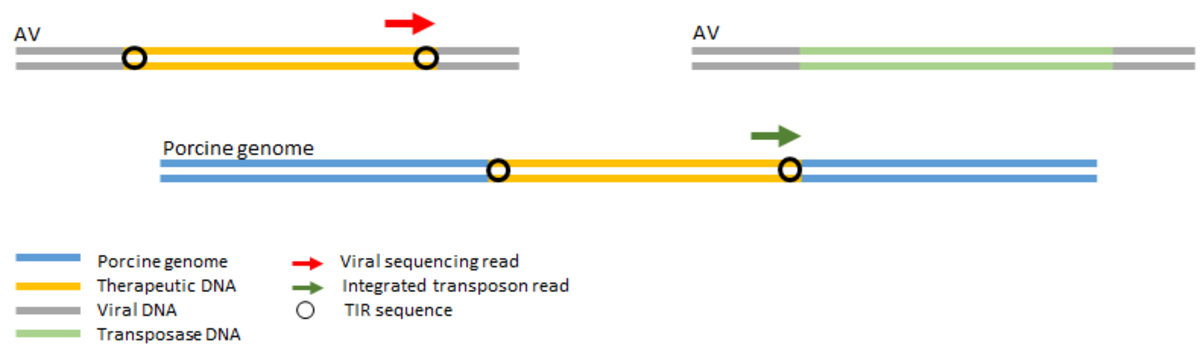
\includegraphics{project_files/figure-latex/Figure1-1.pdf}

\newpage

\section{Attrition of sequencing
reads}\label{attrition-of-sequencing-reads}

Table 1 below details the attrition of sequencing reads where technical
replicates have been combined. The unusally high number of reads that do
not match the transposon vector and which do not align to the susScr3
reference genome requires additional investigation.

Sequencing reads originating from the 3' end of the targeted transposons
were clustered with a sequence identity threshold of 90\% and the 20
most abundant clusters which include 84.1\% of sequenceing reads are
shown in Figure 2. The 20 sequence clusters, except for cluster 18
(possibly from Candidatus Fluviicola) and cluster 20 (no clear source),
map to different adenovirus sequence variants. The representative
sequence for each cluster is provided in Table S1. Alternatively, this
observation can be appreciated by reviewing the most frequent read
sequences and how they align to one another (Table S2).

\vspace{0.25cm}

\begingroup\fontsize{10}{12}\selectfont
\rowcolors{2}{white}{gray!6}

\begin{longtable}[t]{llllll}
\caption{\label{tab:runStats}Table 1. INSPIIRED pipeline read attrition}\\
\hiderowcolors
\toprule
Subject & Sample & Filtered reads & Non-vector like reads & Reads aligning to genome & intSites (reps. combined)\\
\midrule
\endfirsthead
\caption[]{Table 1. INSPIIRED pipeline read attrition \textit{(continued)}}\\
\toprule
Subject & Sample & Filtered reads & Non-vector like reads & Reads aligning to genome & intSites (reps. combined)\\
\midrule
\endhead
\
\endfoot
\bottomrule
\endlastfoot
\showrowcolors
p1166 & Trachea & 923939 & 29430 & 208 & 23\\
p1166 & Lung & 1319372 & 56023 & 50 & 44\\
p1168 & Trachea & 977030 & 355806 & 4 & 4\\
p1168 & Lung & 1201110 & 214530 & 16 & 15\\
p1169 & Trachea & 1289543 & 157285 & 8183 & 36\\
p1169 & Lung & 387593 & 14122 & 2677 & 7\\
p1171 & Trachea & 1052996 & 72905 & 5492 & 86\\
p1171 & Lung & 1130648 & 855182 & 31 & 13\\
p9846 & Trachea & 1130931 & 61204 & 1123 & 13\\
p9850 & Trachea & 680004 & 28962 & 491 & 19\\
p9851 & Trachea & 962963 & 145217 & 402 & 4\\*
\end{longtable}

\rowcolors{2}{white}{white}\endgroup{}

\vspace{0.25cm}

\emph{Figure 2. Most abundant clusters of similar reads (90\% seq id)
with cumulative percentages of all reads.}\\
\vspace{0.25cm}
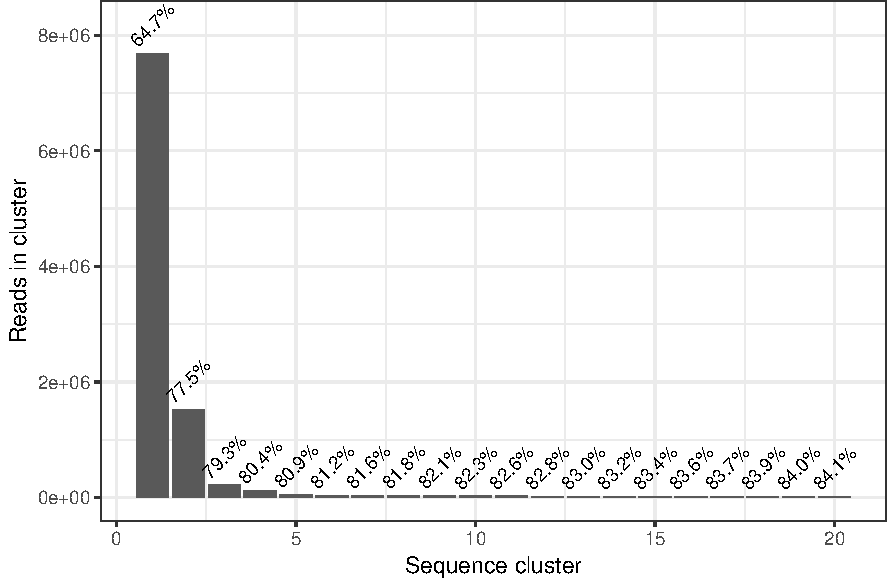
\includegraphics{project_files/figure-latex/readClusters90-1.pdf}
\newpage

\section{Characterization of identified integration
sites}\label{characterization-of-identified-integration-sites}

Figure 3 below shows the distribution of integration sites across the
porcine genome while Figure 4 shows the upstream and downstream
consensus sequence motifs adjacent to those sites. Differences between
the genomic environments of identified sites and the same number of
randomly selected sites from a published lentiviral trial to correct
Wiskott-Aldrich syndrome (WAS) from which no adverse events have been
reported is shown as a heat map in Figure S1\textsuperscript{2}.

The TTAA motif immediately following the identified sites (20.6\% of
sites) was expected given transposase's affinity for this sequence
though the AGGG motif immediately upstream (33.7\% of sites) was not
expected. This finding suggests that a number of integration sites may
be false positives arising from mis-priming against endogenous
piggyBac/LOOPER elements in the porcine genome which are known to end in
AGGG.

\vspace{0.25cm}

\emph{Figure 3. Distriubtion of identified integration sites.}

\vspace{0.50cm}

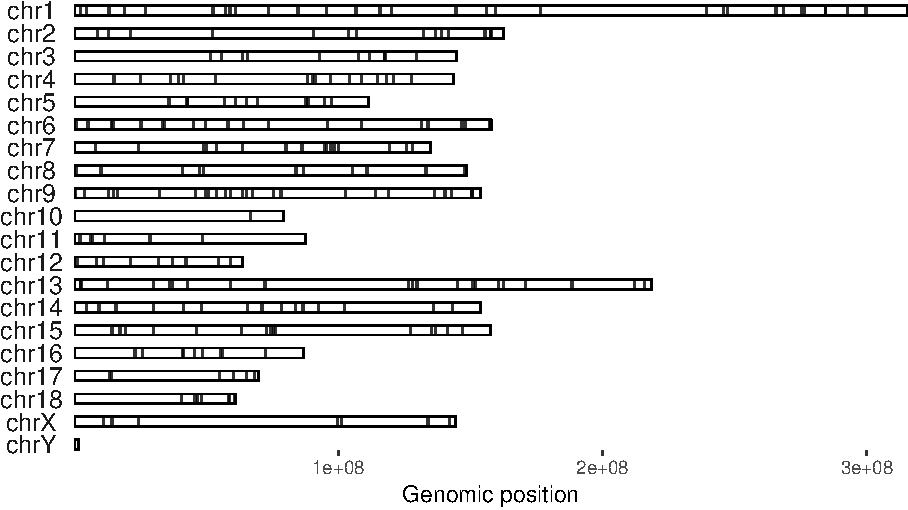
\includegraphics{project_files/figure-latex/intSiteLocPlot-1.pdf}
\vspace{0.50cm}

\emph{Figure 4.}\\
\emph{Concensus upstream (pos. 1-12) and downstream (pos. 13-24)
sequence motifs adjacent to integration sites.}\\
\vspace{0.25cm}
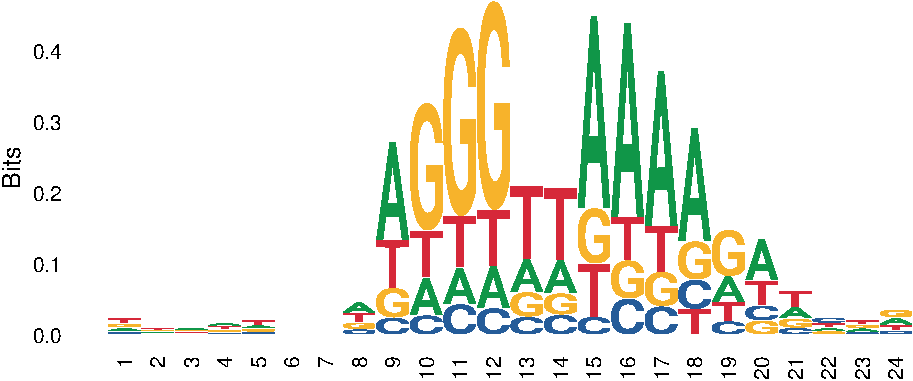
\includegraphics{project_files/figure-latex/upStreamDownStreamLogo-1.pdf}
\newpage

\textbf{Suplimentary figures and tables}

\vspace{1.0cm} \emph{Figure S1.}\\
\emph{ROC heatmap comparing the genomic environments of integration
sites found in this analysis to those found in a published lentiviral
study}

\vspace{1.0cm}

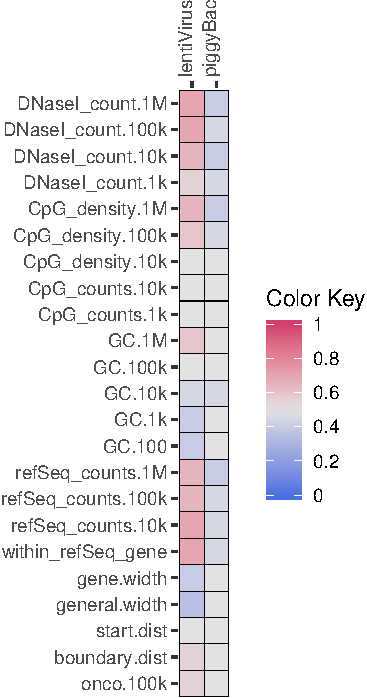
\includegraphics{project_files/figure-latex/FS1-1.pdf}

\newpage

\begingroup\fontsize{10}{12}\selectfont
\rowcolors{2}{white}{gray!6}

\begin{longtable}[t]{ll}
\caption{\label{tab:clusterRepsSeqs}Table S1. Sequence representatives from the most abundant read clusters.}\\
\hiderowcolors
\toprule
Cluster & Representative.sequence\\
\midrule
\endfirsthead
\caption[]{Table S1. Sequence representatives from the most abundant read clusters. \textit{(continued)}}\\
\toprule
Cluster & Representative.sequence\\
\midrule
\endhead
\
\endfoot
\bottomrule
\endlastfoot
\showrowcolors
Cluster 1 & TTAAAAGATCTGGAAGGTGCTGAGGTCCGATGAGACCCGCACCAGGTGCA\\
Cluster 2 & ATTAATACGCAGATCTGGAAGGTGCTGAGGTACGATGAGACCCGCACCAG\\
Cluster 3 & TTAAAAGATCTGGAAGGTGCTGAGGTACGATGAGAAGTCCCTTAAGCGGA\\
Cluster 4 & TTAAAAGATCTGGAAGGTGCTGAGGTACGATGAGACCCGCACCAGTCCCT\\
Cluster 5 & TTAAAAGATCTGGAAGGTGCTGAGGTACGAGTCCCTTAAGCGGAGGCTAC\\
Cluster 6 & CTAAAAGAGCTGGAAGGTGCTGAGGTACGATAAGACCCGAACCAGGTGCA\\
Cluster 7 & ATTAATACGCAGATCTGGAAGGTGCTGAGGTACGATGGGTCCCTTAAGCG\\
Cluster 8 & ATTAATACGCAGATCTGGAAGGTGCTGAGGTACGATGAGACCCGGGTCCC\\
Cluster 9 & TTAAAAGATCTGGAAGGTGCTGAGGTAAGTCCCTTAAGCGGAGTAAATCG\\
Cluster 10 & TTAAAAGATCTGGAAGGTGCTGAGGTAGTCCCTTAAGCGGAGGTCGGCCG\\
Cluster 11 & TTAAAGGATCTGGAAGGTGCTGAGGTACGGTGAGACCAGCACCGGGTGCA\\
Cluster 12 & TTAAAAGCTCTGGAAGGTGCTGCGGTACGATGCGACCAGCCCCAGGTGCA\\
Cluster 13 & ATTAATACGCAGATCTGGAAGGTGCTGAGGTAGTCCCTTAAGCGGAGACC\\
Cluster 14 & TTAAAAGATCCGGAAGGTGCTGAGGCAAGATGAGACCCGCACTAGGTGCA\\
Cluster 15 & TTAAAAGGTCTGTAAGGCGCTGAGGTACGCTGAGACCCGCACCAGGTGCA\\
Cluster 16 & TTAAAAGATCTGGAAGGTGCTGAGGTACGAGGTCCCTTAAGCGGAGAGCC\\
Cluster 17 & TTAAAAGACCTGGAAGGTGCTGAGGTACGCTGAGACTCGCCCCAGGTGCA\\
Cluster 18 & AGGCTCCGGTTGATTTGACTGCCGACAATTACCATAGCGTCAGTCCTGGT\\
Cluster 19 & GTAACAGATCTGGAAGGTGCTGAGGGACGATGAGACCCGCACAAGGTGCA\\
Cluster 20 & TTGTTGGCCGGGGCTGAGACTCGTTACATAGAACAATTACCATAGCGTCA\\*
\end{longtable}

\rowcolors{2}{white}{white}\endgroup{}

\vspace{1.0cm}

\begingroup\fontsize{10}{12}\selectfont
\rowcolors{2}{white}{gray!6}

\begin{longtable}[t]{>{\ttfamily\raggedright\arraybackslash}p{37em}>{\ttfamily\raggedright\arraybackslash}p{4em}>{\ttfamily\raggedright\arraybackslash}p{3em}>{\ttfamily\raggedright\arraybackslash}p{4em}>{\ttfamily\raggedright\arraybackslash}p{4em}}
\caption{\label{tab:genomicSeqFreqTable_aligned}Table S2. Most abundant transposon 3' reads (ITR seqs removed)}\\
\hiderowcolors
\toprule
Genomic sequence & nReads & Cumm. \%reads & Transpon vector position & Transposase vector position\\
\midrule
\endfirsthead
\caption[]{Table S2. Most abundant transposon 3' reads (ITR seqs removed) \textit{(continued)}}\\
\toprule
Genomic sequence & nReads & Cumm. \%reads & Transpon vector position & Transposase vector position\\
\midrule
\endhead
\
\endfoot
\bottomrule
\endlastfoot
\showrowcolors
ATTAATACGCAGATCTGGAAGGTGCTGAGGTACGATGAGACCCGCACCAG & 1305206 & 67.12 & NA & NA\\
TTAAAAGAG-----CTGGAAGGTGCTGAGGTACGATGAGACCCGCACCAGGTGCA & 36877 & 67.43 & 2997 & NA\\
TTAAAAGAT-----CTGGAAGGTGCTGAGGTACGATGAGACCC-----AGTCCCTTAAGC & 32231 & 67.70 & NA & NA\\
TTAAAAGAT-----CTGGAAGGTGCTGAGGTACGATGAGACCCGCACCAGTCCCT & 31541 & 67.97 & NA & NA\\
TTAAAAGAT-----CTGGAAGGTGCTGAGGTACGATGAGACCCGCACCAGGTGCG & 28122 & 68.21 & 2997 & NA\\
CTAAAAGAT-----CTGGAAGGTGCTGAGGTACGATGAGACCCGCACCAGGTGCA & 27473 & 68.44 & 2997 & NA\\
TTAAAAGAT-----CTGGAAGGTGCTGAGGCACGATGAGACCCGCACCAGGTGCA & 26538 & 68.66 & 2997 & NA\\
TTAAAAGAT-----CTGGAGGGTGCTGAGGTACGATGAGACCCGCACCAGGTGCA & 26425 & 68.88 & 2997 & NA\\
TTAAAAGAT-----CTGGAAGGTGCTGAGGTACGATGAGACCCGCACCAGGTGTA & 26348 & 69.10 & 2997 & NA\\
TTAAAAGAT-----CTGGAAGGTGCTGAGGTACGATGAGACCCGCACCAGGCGCA & 25893 & 69.32 & 2997 & NA\\
TTAAAGGAT-----CTGGAAGGTGCTGAGGTACGATGAGACCCGCACCAGGTGCA & 25378 & 69.53 & 2997 & NA\\
TTAAAAGAT-----CTGGAAGGTGCTGAGGTACGATGAGGCCCGCACCAGGTGCA & 24603 & 69.74 & 2997 & NA\\
TTAAAAGAT-----CTGGAAGGTGCTGAGGTACGATGAGACC-------AGTCCCTTAAGCG & 23819 & 69.94 & NA & NA\\
TTAAAAGAT-----CTGGAAGGTGCCGAGGTACGATGAGACCCGCACCAGGTGCA & 23700 & 70.14 & 2997 & NA\\
TTAAAAGAT-----CTGGAAGGTGCTGAGGTACGATGGGACCCGCACCAGGTGCA & 22740 & 70.33 & 2997 & NA\\
TTAAAAGCT-----CTGGAAGGTGCTGAGGTACGATGAGACCCGCACCAGGTGCA & 22651 & 70.52 & 2997 & NA\\
TTAAAAGAT-----CTGGAAGGTGCTGAGGTACGATGAGACCCGCACCAGGTAGT & 22234 & 70.71 & NA & NA\\
TTAAAAGAT-----CTGGAAGGCGCTGAGGTACGATGAGACCCGCACCAGGTGCA & 22124 & 70.90 & 2997 & NA\\
TTAAAAGAT-----CTGGAAGGTGCTGAGGTACGATGAGACCCGC----AGTCCCTTAA & 21821 & 71.08 & NA & NA\\
TTAAAAGAT-----CTGGAAGGTGCTGAGGTACGATGAGACCCGCACCGGGTGCA & 21630 & 71.26 & 2997 & NA\\
TTAAAAGAT-----CCGGAAGGTGCTGAGGTACGATGAGACCCGCACCAGGTGCA & 21112 & 71.44 & 2997 & NA\\
TTAAAAGAT-----CTGGAAGGTGCTGAGGTACGATGAGACCCGCGCCAGGTGCA & 20804 & 71.62 & 2997 & NA\\
TTACAAGAT-----CTGGAAGGTGCTGAGGTACGATGAGACCCGCACCAGGTGCA & 20361 & 71.79 & 2997 & NA\\
TTAAAAGGT-----CTGGAAGGTGCTGAGGTACGATGAGACCCGCACCAGGTGCA & 20337 & 71.96 & 2997 & NA\\
TTAAAAGAT-----CTGGAAGGTGCTGAGGTACGACGAGACCCGCACCAGGTGCA & 20153 & 72.13 & 2997 & NA\\
TTAAAAGAT-----CTGGAAGGTGCTGAGGTACGATGAGACCCGCACCAGGTGAG & 19495 & 72.29 & 2997 & NA\\
TTAAAAGAT-----CTGGAAGGTGCTGAGGTGCGATGAGACCCGCACCAGGTGCA & 18282 & 72.44 & 2997 & NA\\
TTAAAAGAT-----CTGGAAGGTGCTGAGGTACGATGAG----------AGTCCCTTAAGCGGAG & 18216 & 72.59 & NA & NA\\
TTAAAAGAT-----CTGGAAGGTGCTGGGGTACGATGAGACCCGCACCAGGTGCA & 17542 & 72.74 & 2997 & NA\\
TTAAAAGAT-----CTGGAAGGTGCTGAGGTACGATGAGAC--------AGTCCCTTAAGCGG & 17337 & 72.89 & NA & NA\\
TTAAAAGAT-----CTGGAAGGTGCTGAGGTACGATGAGACCCG-----AGTCCCTTAAG & 16814 & 73.03 & NA & NA\\
TTAAAAGAC-----CTGGAAGGTGCTGAGGTACGATGAGACCCGCACCAGGTGCA & 16457 & 73.17 & 2997 & NA\\
TTAAAAGAT-----CTGGAAGGTGCTGAGGTACGGTGAGACCCGCACCAGGTGCA & 16137 & 73.31 & 2997 & NA\\
TTAGAAGAT-----CTGGAAGGTGCTGAGGTACGATGAGACCCGCACCAGGTGCA & 15674 & 73.44 & 2997 & NA\\
TTAAAAGAT-----CTGGAAGGTGCTGAGGTACGATGAGACCCGCACCAAGTCCC & 15558 & 73.57 & NA & NA\\
TTAAAAGAT-----CTGGAAGGTGCTGAGGTACGATGAGACCCGCACCAGGAGTC & 14669 & 73.69 & NA & NA\\
AGGCTCCGGTTGATTTGACTGCCGACAATTACCATAGCGTCAGTCCTGGT & 14610 & 73.81 & NA & NA\\
TTAAAAGAT-----CTGGAAGGTGCTGAGGTACGATGAGACCCACACCAGGTGCA & 14587 & 73.93 & 2997 & NA\\
TTAAAAGAT-----CTGGAAGGTGCTGAGGTACGATGAGACTCGCACCAGGTGCA & 14204 & 74.05 & 2997 & NA\\
TTAACAGAT-----CTGGAAGGTGCTGAGGTACGATGAGACCCGCACCAGGTGCA & 13511 & 74.16 & 2997 & NA\\
TTAAAAGAT-----CTGGAAGGTGTTGAGGTACGATGAGACCCGCACCAGGTGCA & 12890 & 74.27 & 2997 & NA\\
TTAAAAGAT-----CTGGGAGGTGCTGAGGTACGATGAGACCCGCACCAGGTGCA & 12311 & 74.37 & 2997 & NA\\
TTAAAAGAT-----CTGGAAGGTACTGAGGTACGATGAGACCCGCACCAGGTGCA & 11687 & 74.47 & 2997 & NA\\
TTAAAAGAT-----CTGGAAGGTGCTGAGGTACGATGAGACCCGTACCAGGTGCA & 11611 & 74.57 & 2997 & NA\\
TTAAAAGAT-----CTGGAAGGTGCTGAGGTATGATGAGACCCGCACCAGGTGCA & 11530 & 74.67 & 2997 & NA\\
TTAAAAGAT-----CTGGAAGGTGCTGAGGTACGATGAGACCCGCACCAGAGTCC & 11391 & 74.77 & NA & NA\\
TTAAAAGAT-----CTGGAAGGTGCTGAGGTACGATGAGACCCGCACCAGGTACA & 11172 & 74.86 & 2997 & NA\\
TTAAAAGAT-----CTGGAAGGTGCTGAGGTACGATGAGACCTGCACCAGGTGCA & 10666 & 74.95 & 2997 & NA\\
TTAAAAGAT-----CTGGAAGGTGCTGAGGTACGATGAGATCCGCACCAGGTGCA & 10293 & 75.04 & 2997 & NA\\
TTAAAAGAT-----CTGGAAGGTGCTGAGGTACAATGAGACCCGCACCAGGTGCA & 10289 & 75.13 & 2997 & NA\\
TTAAAAGAT-----CTGGAAGGTGCTGAGGTACG---------------AGTCCCTTAAGCGGAGTTACA & 10067 & 75.21 & NA & NA\\
TCAAAAGAT-----CTGGAAGGTGCTGAGGTACGATGAGACCCGCACCAGGTGCA & 9960 & 75.29 & 2997 & NA\\
TTGTTGGCCGGGGCTGAGACTCGTTACATAGAACAATTACCATAGCGTCA & 9338 & 75.37 & NA & NA\\
ATTAATACGCAGATCTGGAAGGTGCTGAGGTACGATGAGACCCGG-----GTCCC & 9275 & 75.45 & NA & NA\\
TTAAAAGAT-----CTGGAAGGTGCTGAGGTACGATGAGACCCGCACCAGATGCA & 8587 & 75.52 & 2997 & NA\\
TTAAAAGAT-----CTGGAAGGTGCTGAGGTACGATGAGACCCGCA---AGTCCCTTA & 8561 & 75.59 & NA & NA\\
TTAAAAGAT-----CTGGAAGGTGCTGAGGTACGATGAGACCCGCATCAGGTGCA & 8504 & 75.66 & 2997 & NA\\
TTTAAAGAT-----CTGGAAGGTGCTGAGGTACGATGAGACCCGCACCAGGTGCA & 8096 & 75.73 & 2997 & NA\\
TTCAAAGAT-----CTGGAAGGTGCTGAGGTACGATGAGACCCGCACCAGGTGCA & 7748 & 75.80 & 2997 & NA\\
TTGAAAGAT-----CTGGAAGGTGCTGAGGTACGATGAGACCCGCACCAGGTGCA & 7705 & 75.86 & 2997 & NA\\
TTAAAAGAT-----CTGGAAGGTGCTGAAGTACGATGAGACCCGCACCAGGTGCA & 7639 & 75.92 & 2997 & NA\\
ATTAATACGCAGATCTGGAAGGTGCTGAGGTACGATGAGA---------AGTCCCTTAA & 7471 & 75.98 & NA & NA\\
TTAAAAGAT-----CTGGAAGGTGCTGAGGTACGATGAGACCCGCAC--AGTCCCTT & 7430 & 76.04 & NA & NA\\
TTAAGAGAT-----CTGGAAGGTGCTGAGGTACGATGAGACCCGCACCAGGTGCA & 7412 & 76.10 & 2997 & NA\\
TTAAAGATC------TGGAAGGTGCTGAGGTACGATGAGACCCGCACCAGGTGCAG & 7287 & 76.16 & 2998 & NA\\
ATTAATACGCAGATCTGGAAGGTGCTGAGGTACGATGAGACCCGC----AGTCC & 7174 & 76.22 & NA & NA\\
TTATAAGAT-----CTGGAAGGTGCTGAGGTACGATGAGACCCGCACCAGGTGCA & 7074 & 76.28 & 2997 & NA\\
ATTAATACGCAGATCTGGAAGGTGCTGAGGTACGACGAGACCCGCACCAG & 6883 & 76.34 & NA & NA\\
TTAAAAGAT-----CTGGAAGGTGCTGAGGTACGATGAGA---------AGTCCCTTAAGCGGA & 6807 & 76.40 & NA & NA\\
TTAAAAGAT-----CTGGAAGGTGCTGAGGTACGATGAGACCCGCACTAGGTGCA & 6762 & 76.46 & 2997 & NA\\
TTAAAAGAT-----CTGGAATGTGCTGAGGTACGATGAGACCCGCACCAGGTGCA & 6611 & 76.52 & 2997 & NA\\
ATTAATACGCAGATCTGGAAGGTGCTGAGGTACGATGAG----------AGTCCCTTAAG & 6453 & 76.57 & NA & NA\\
ATTAATACGCAGATCTGGAAGGTGCTGAGGTACGATGAGACCCG-----AGTCCC & 6401 & 76.62 & NA & NA\\
ATTAATACGCAGATCTGGAAGGCGCTGAGGTACGATGAGACCCGCACCAG & 6265 & 76.67 & NA & NA\\
TTAAAAGAT-----TTGGAAGGTGCTGAGGTACGATGAGACCCGCACCAGGTGCA & 6098 & 76.72 & 2997 & NA\\
ATTAATACGCAGATCTGGAAGGTGCTGAGGTACGATGAGAC--------AGTCCCTTA & 6001 & 76.77 & NA & NA\\
ATTAATACGCAGATCTGGAAGGTGCTGAGGCACGATGAGACCCGCACCAG & 5965 & 76.82 & NA & NA\\
TTAAAAGAT-----CTGGAAGGTGCTGTGGTACGATGAGACCCGCACCAGGTGCA & 5924 & 76.87 & 2997 & NA\\
TTAAAAGAT-----CTGGAAGGTGCTGAGGTACGATGAGACCCGCACCAAGTGCA & 5582 & 76.92 & 2997 & NA\\
TTAAAAGAT-----CTGGAAGATGCTGAGGTACGATGAGACCCGCACCAGGTGCA & 5421 & 76.97 & 2997 & NA\\
TTAAAAGAT-----CTGGAAAGTGCTGAGGTACGATGAGACCCGCACCAGGTGCA & 5359 & 77.02 & 2997 & NA\\
TTAAAAGAT-----CTGAAAGGTGCTGAGGTACGATGAGACCCGCACCAGGTGCA & 5265 & 77.06 & 2997 & NA\\
ATTAATACGCAGATCTGGAAGGTGCTGAGGTACGAT-------------AGTCCCTTAAGCGG & 5225 & 77.10 & NA & NA\\
TTAAAAGAT-----CTGGAAGGTGCTGAGGTACGATGAGACCCGCACCTGGTGCA & 5028 & 77.14 & 2997 & NA\\
ATTAATACGCAGATCTGGAGGGTGCTGAGGTACGATGAGACCCGCACCAG & 4972 & 77.18 & NA & NA\\
ATTAATACTCAGATCTGGAAGGTGCTGAGGTACGATGAGACCCGCACCAG & 4970 & 77.22 & NA & NA\\
ATTAATACGCAGATCCGGAAGGTGCTGAGGTACGATGAGACCCGCACCAG & 4866 & 77.26 & NA & NA\\
TTAAACGAT-----CTGGAAGGTGCTGAGGTACGATGAGACCCGCACCAGGTGCA & 4796 & 77.30 & 2997 & NA\\
TTAAAAGAT-----CTGGAAGGTGCTGAGATACGATGAGACCCGCACCAGGTGCA & 4778 & 77.34 & 2997 & NA\\
ATTAATACGCAGATCTGGAAGGTGCTGAGGTACGATGAGGCCCGCACCAG & 4775 & 77.38 & NA & NA\\
TTAAAAGAT-----CTGGAAGGTGCTAAGGTACGATGAGACCCGCACCAGGTGCA & 4681 & 77.42 & 2997 & NA\\
TTAAAAGAT-----CTAGAAGGTGCTGAGGTACGATGAGACCCGCACCAGGTGCA & 4647 & 77.46 & 2997 & NA\\
ATTAATACGCAGATCTGGAAGGTGCTGAGGTACGATGAGACC-------AGTCCCTT & 4608 & 77.50 & NA & NA\\
ATTAATACGCAGATCTGGAAGGTGCCGAGGTACGATGAGACCCGCACCAG & 4595 & 77.54 & NA & NA\\
TTAAAAGAT-----CTGGTAGGTGCTGAGGTACGATGAGACCCGCACCAGGTGCA & 4551 & 77.58 & 2997 & NA\\
ATTAATACGCAGATCTGGAAGGTGCTGAGGTAAGATGAGACCCGCACCAG & 4512 & 77.62 & NA & NA\\
TTAAAAGAT-----CTGGAAGGTGCTGAGGTACGATGCGACCCGCACCAGGTGCA & 4469 & 77.66 & 2997 & NA\\
TTAAAAGAT-----CTGGACGGTGCTGAGGTACGATGAGACCCGCACCAGGTGCA & 4431 & 77.70 & 2997 & NA\\
TTAAAAGAT-----CTGGAAGGTGCTGAGGTACGATAAGACCCGCACCAGGTGCA & 4373 & 77.74 & 2997 & NA\\*
\end{longtable}

\rowcolors{2}{white}{white}\endgroup{}

\newpage

\textbf{References}

\begin{enumerate}
\def\labelenumi{\arabic{enumi}.}
\tightlist
\item
  INSPIIRED: A Pipeline for Quantitative Analysis of Sites of New DNA
  Integration in Cellular Genomes. Sherman E, Nobles C, Berry CC, et al.
  Molecular Therapy Methods \& Clinical Development. 2017;4:39-49.
  \url{doi:10.1016/j.omtm.2016.11.002}.
\end{enumerate}

\vspace{0.10cm}

\begin{enumerate}
\def\labelenumi{\arabic{enumi}.}
\setcounter{enumi}{1}
\tightlist
\item
  Outcomes following gene therapy in patients with severe
  Wiskott-Aldrich syndrome. Hacein-Bey Abina S, Gaspar HB, Blondeau J,
  Caccavelli L, Charrier S, Buckland K, Picard C, Six E, Himoudi N,
  Gilmour K, McNicol AM, Hara H, Xu-Bayford J, Rivat C, Touzot F,
  Mavilio F, Lim A, Treluyer JM, Héritier S, Lefrère F, Magalon J,
  Pengue-Koyi I, Honnet G, Blanche S, Sherman EA, Male F, Berry C,
  Malani N, Bushman FD, Fischer A, Thrasher AJ, Galy A, Cavazzana M.
  JAMA. 2015 Apr 21;313(15):1550-63.
\end{enumerate}


\end{document}
